\documentclass[12pt,letterpaper,noanswers]{exam}
\usepackage[usenames,dvipsnames,svgnames,table]{xcolor}
\usepackage[margin=0.9in]{geometry}
\renewcommand{\familydefault}{\sfdefault}
\usepackage{multicol}
\pagestyle{head}
\header{AM 108 Class 12}{}{Conservative system (page \thepage)}
\runningheadrule
\headrule

\usepackage{graphicx} % more modern
\usepackage{amsmath} 
\usepackage{amssymb} 

\usepackage{hyperref}
\usepackage{tcolorbox}

\begin{document}
 \pdfpageheight 11in 
  \pdfpagewidth 8.5in

\noindent 





\begin{itemize}
\itemsep0em
    \item There is a problem set due Friday Oct 2nd.
    \item There will be a two question skill check on Friday.  The question info is below.
    \item There is not a pre-class assignment for Friday.
    \item Find office hours info on the Canvas page.
\end{itemize}

\hrule
\vspace{0.2cm}





\noindent\textbf{Teams}

\begin{multicols}{2}
1. 

\end{multicols}

\noindent \textbf{Teams 3 and 4}: Post screenshots of your work to the course Google Drive today.  Include words, labels, and other short notes that might make those solutions useful to you or your classmates.  Find the link in Canvas (or here: \url{https://drive.google.com/drive/u/0/folders/1GcpwvKHD4tMecpFQ4lNxN_r5Ylj7YHbd})


\vspace{0.2cm}
\hrule
\vspace{0.2cm}

\noindent\textbf{Extra facts/vocab}

\begin{tcolorbox}
A conservative system does not have attracting or repelling fixed points.  Instead, fixed points might be saddle points, nonlinear centers, or non-isolated.

A \textbf{homoclinic orbit} is a trajectory that starts and ends at a single fixed point.

A \textbf{heteroclinic orbit} is a trajectory that connects two fixed points.
\end{tcolorbox}

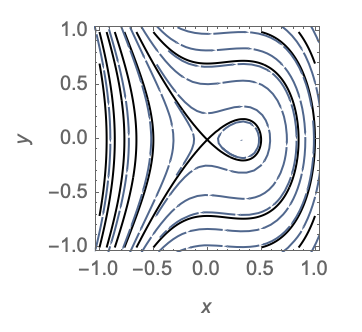
\includegraphics[scale=0.9]{img/C12homoclinic.png}
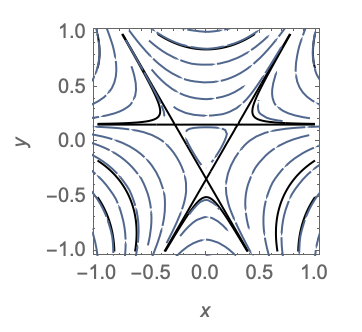
\includegraphics[scale=0.9]{img/C12heteroclinic.png}

\noindent\textbf{Three ways to find a conserved quantity}
\begin{tcolorbox}
Consider a system of the form $m\ddot x = F(x)$ where $F(x) = -\dfrac{dV}{dx}$ with $V(x)$ called the \textbf{potential energy}.  $E = \frac{1}{2}m\dot x^2 + V$ is a conserved quantity for this system.

A \textbf{phase curve} of a system $\dot x = f(x,y), \dot y = g(x,y)$ is a curve $y = Y(x)$ (note that $\dot y = Y_x \dot x$) that obeys the differential equation $\frac{dY}{dx} = \frac{\dot y}{\dot x} = \frac{g(x,Y)}{f(x,Y)}$.  Trajectories that start on such a curve stay on it.  When $\frac{dy}{dx} = \frac{g(x,y)}{f(x,y)}$ is a separable differential equation, the process of solving it can also yield a conserved quantity.

A \textbf{Hamiltonian} function, $H(x,y)$ is an energy function.  The associated dynamical system $\dot x = \frac{\partial H}{\partial y}$, $\dot y = -\frac{\partial H}{\partial x}$ is called a \textbf{Hamiltonian system}.  In a Hamiltonian system, the Hamiltonian is a conserved quantity.


\end{tcolorbox}

\vspace{0.2cm}
\hrule
\vspace{0.2cm}

\noindent\textbf{Examples: finding a conserved quantity}

\begin{questions}
\item Let $\ddot x = x^3$.  By introducing $y = \dot x$, this can be written as the system $\dot x = y, \dot y = x^3$.

$V(x) = -\int x^3 dx = -x^4/4$.  Try $E = \frac{1}{2}y^2 - x^4/4$.  Is this conserved?  (It should be).

$\frac{dE}{dt} = y\dot y - x^3\dot x = yx^3 - x^3y = 0$.  It is conserved!

\item\begin{parts}
 \item The model nondimensionalizes to 
  \begin{align*}
 x' = & x - x y \\
 y' = &y(\rho - x).
 \end{align*}
 \emph{This nondimensionalization requires assuming that each population has its own units, so number of rabbits and number of sheep were each be assigned their own unknown constant in the nondimensionalization process.}

Using the nondimensional system, find an expression satisfied by most phase curves.  %show that almost all trajectories have phase curves of the form $\rho \ln x - x = \ln y -y + C$.
 \emph{Solve a separable differential equation to do this.  You don't need to write it in the form $y = Y(x)$; an implicit relationship between $x$ and $y$ is fine.}
 
 \item Argue that the quantity $H(x,y) = y - \ln y + \rho \ln x - x$ is almost always conserved.
 
 \textit{Which trajectories don't work with this function?}

\end{parts}

\item Let $\dot x = x^2, \dot y = -2xy + x$.  This system is Hamiltonian.

Assume $H_y = x^2$, so $H = x^2 y + g(x)$ where $g(x)$ is unconstrained by $H_y$.

Using this $H$, compute $H_x$ to find $H_x = 2xy + g'(x)$.  We want $-\dot y = H_x$, so $-2xy + x = -2xy - g'(x)$.  This implies that $g'(x) = -x$, so $g(x) = -x^2/2 + c$.  We can choose $c = 0$ for simplicity.

So we have $H(x,y) = x^2y - x^2/2$ as a conserved quantity.

\end{questions}
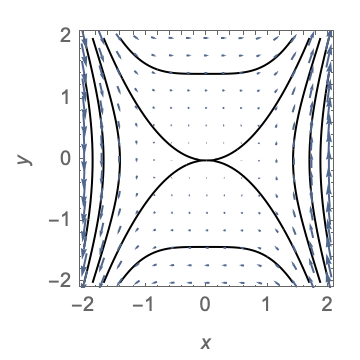
\includegraphics[scale=0.9]{img/C12conservative-p3.png}
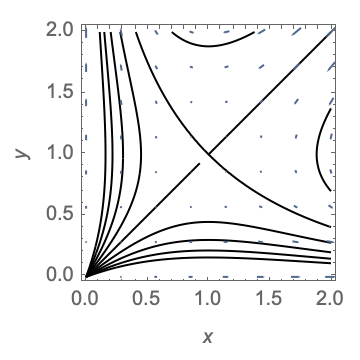
\includegraphics[scale=0.9]{img/C12conservative-p2.png}
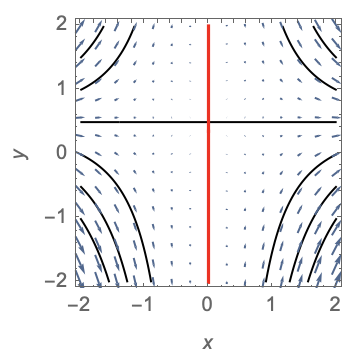
\includegraphics[scale=0.9]{img/C12conservative-p1.png}


\vspace{0.2cm}
\hrule
\vspace{0.2cm}

\noindent\textbf{Skill Check C13 practice}
\begin{questions}

\item Retake of Skill Check C10 on classifying fixed points of a linear system based on $\tau$ and $\Delta$.  See the C09 handout for the sample question.

\item Let $H(x,y) = xy$ be a conserved quantity for a 2D dynamical system.  Use this information to sketch three phase curves of the system.
\end{questions}

\vspace{0.2cm}

\hrule
\vspace{0.2cm}

\noindent\textbf{Skill Check C13 practice solution}

Phase curves are curves $y=Y(x)$ such that a trajectory that starts on the curve stays on the curve.

Every contour curve $H(x,y) = c$ is such a curve.  Start with $H(x,y) = 0$, so $xy = 0$.  $y = 0$ is a phase curve.  $xy = 1 \Rightarrow y = 1/x$ is another.  $y = 2/x$ is a third.

I'll sketch these three curves in the $xy$-plane.

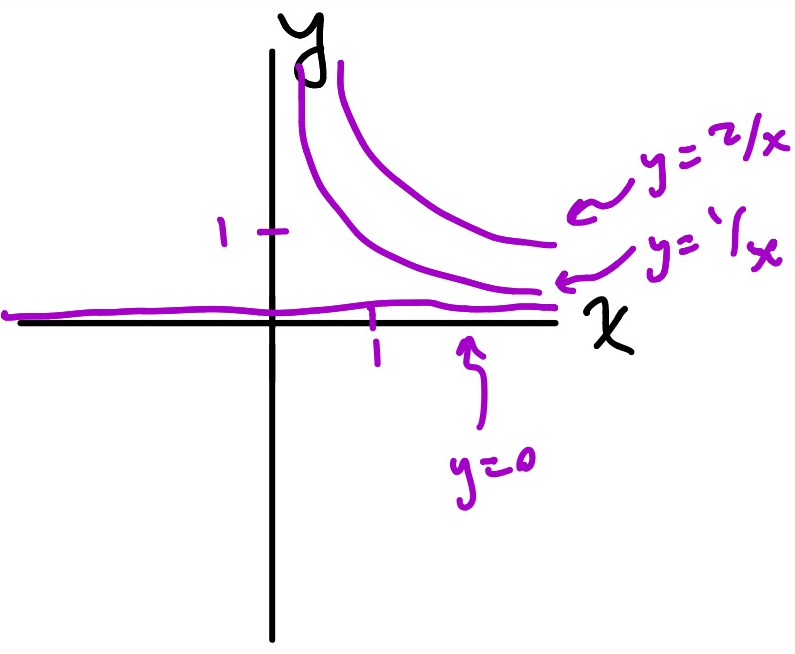
\includegraphics[width=3in]{img/C12curves.png}

\vspace{0.2cm}
\hrule
\vspace{0.2cm}



\begin{questions}
\setcounter{question}{-1}
\item If you were trapped on an island, what are two items/people that you'd want to have along?  Why?

\item  Consider the system 
 \begin{align*}
 \dot{x} = & - \mu y + x y   \\
 \dot{y} = &\ \mu x + \frac{1}{2}(x^2 - y^2).
 \end{align*}
 Assume $\mu > 0$.
 
 \begin{parts}
 \item This system has a conserved quantity.  Assume $\dot x = H_y$ and $\dot y = -H_x$ for an unknown function $H(x,y)$.  If our assumption is correct then $\partial_x\dot x = -\partial_y \dot y$.  Why is that?
 \item Show that $\partial_x\dot x = -\partial_y \dot y$ for this system.
 \item Construct a function $H(x,y)$ that is conserved for this system.
 \item If time permits, begin the process of constructing a phase portrait for this system.
 \end{parts}
\end{questions}

\eject
\textbf{Answers}: 

1a: Mixed partials are equal, $H_{xy} = H_{yx}$, so if $\dot x$ and $\dot y$ are given by those partials, then we can use $\dot x$ and $\dot y$ to compute the mixed partials in two different ways.

1b: $\partial_x\dot x = y$.  $-\partial_y\dot y = -\frac{1}{2}(-2y) = y$.  These are equal.

1c: $H_y = -\mu y + xy$ so $H(x,y) = \frac{1}{2}y^2(-\mu + x) + G(x)$.  $-H_x = -\frac{1}{2}y^2 - G_x =\mu x + \frac{1}{2}(x^2 - y^2)$ so $G_x = -\mu x - \frac{1}{2}x^2$.  $G(x) = -\mu\frac{1}{2}x^2 - \frac{1}{6}x^3 + c$.  I just need a single function that works, not a whole family of them.  $H(x,y) = -\mu\frac{1}{2}x^2 - \frac{1}{6}x^3+\frac{1}{2}y^2(-\mu + x) $ is one such function.

\end{document}